\documentclass{report}
 \usepackage{lipsum}
 \usepackage[margin=1in,left=1.5in,includefoot]{geometry}
\usepackage{graphicx} %allows you to get photos 
\usepackage{float} 
\usepackage{blindtext}
\usepackage[utf8]{inputenc}
\usepackage{wrapfig,lipsum}
\usepackage{parallel,enumitem}
\usepackage{hyperref}
\usepackage{listings}

\usepackage[T1]{fontenc}
\usepackage{inconsolata}

\usepackage{color}

\definecolor{pblue}{rgb}{0.13,0.13,1}
\definecolor{pgreen}{rgb}{0,0.5,0}
\definecolor{pred}{rgb}{0.9,0,0}
\definecolor{pgrey}{rgb}{0.46,0.45,0.48}

\usepackage{listings}
\lstset{language=Java,
  showspaces=false,
  showtabs=false,
  breaklines=true,
  showstringspaces=false,
  breakatwhitespace=true,
  commentstyle=\color{pgreen},
  keywordstyle=\color{pblue},
  stringstyle=\color{pred},
  basicstyle=\ttfamily,
  moredelim=[il][\textcolor{pgrey}]{$$},
  moredelim=[is][\textcolor{pgrey}]{\%\%}{\%\%}
}




\begin{document}


\begin{titlepage}
	\centering
	
\includegraphics[width=15cm,height=4cm]{images/ibr.png}\par\vspace{1cm}
	{\scshape\LARGE  \par}
	\vspace{1cm}
	{\scshape\Large Research Project\par}
	\vspace{1.5cm}
	{\huge\bfseries Trustworthy Recording of Media Files Using Blockchains \par}
	\vspace{1cm}
	{\huge\itshape Hesham Hosney\par}
        \vspace{2cm} 
	{\Large Supervisor:\par } 
	{\huge Prof. Dr. Rüdiger Kapitza\par}
        \vspace{.5cm} 
        {\huge M.Sc. Signe Rüsch}
	\vfill
% Bottom of the page
	{\large \today\par}
\end{titlepage}


\cleardoublepage
\tableofcontents
\listoffigures
\cleardoublepage



\begin{abstract}
The Blockchain technology is having a huge potential since it had a huge contribution in redefining the way the data is stored, updated, and moved.
It is expected that the blockchain will revolutionize different business and industry with such huge capabilities,
In this report, we proposed a platform for detecting Fake news using Hypereledger fabric technology.
We implemented an Android application that allows the users to share and rank nearby events.  \\ 

The event is an incident which happened somewhere, for example, a car accident or urgent road maintenance leads to closing the main road. We incent users to share their stories and the stories will be displayed only to the nearby users.
We proposed a reputation system for ranking the users and their stories. The algorithm ranks the users and the events they created is based on the users' location or how close the users from an event they are judging, and the users' reputation score. \\ 
By keeping a reputation score for every single user depending on his previous contributions to the platform. and how close he was from the event he is assessing furthermore we collect the last 24 hours location traces for every user to make sure that the users are not scamming the platform. using the aforementioned methods we assure the trustworthiness of the shared events.
Thanks to Hyperledger fabrics' features like immutability, trustworthy, and transparency, we proposed a prototype of our application to mitigate the spread of Fake news our application leveraging the blockchain technology and enabling it as a simple use case in the industry.
We assure the data confidentiality since it will be stored on a distributed ledger and only updated by the chaincode which holds the whole business logic modifying the data once it's created is not possible the data will be immutably stored and distributed on multiple nodes.  \\ 

This report describes the proposed work as follow, we will start with the main motivation, a walk through the application and the use case scenario, in chapter 2 we will give a brief introduction about blockchain and Hyperledger fabric. In chapter 3 we discuss the application infrastructure we used, for instance, the network nodes, SDK implementation, and API calls. In Chapter 4 we are summarizing the Android application part and how we designed and developed the application in depth. Chapter 5 will focus on the results and insights gained and issues. 
\end{abstract}
\cleardoublepage
\centerline{\bfseries Statement of Originality}
	\vspace*{1em}
	\noindent
	This research project has been performed independently with the support of my supervisors.
	To the best of the author's knowledge, this research project contains no material previously
	published or written by another person except where due reference is made in the text.

\cleardoublepage
\chapter{Introduction}

	
	
	% \begin{figure}[H]
	%\includegraphics[width=13cm,height=5cm]{/Users/Whosham/Desktop/ICT/report/PIC/3.png}
	%\caption{Let's Encrypt vs Commercial Certificate Authorities}
	%\end{figure}
	 
	 
	\section{Abstract}

The Blockchain technology is having a huge potential since it had a huge contribution in redefining the way the data is stored, updated, and moved.
it is expected that the blockchain will revolutionize different business and industry. with such huge capabilities,
In this report, we proposed a platform for detecting fake news using Hypereledger fabric technology, we implemented an android application in order to, help the users to share and rank nearby events. Thanks to Hyperledger fabrics' features like immutability, trustworthy, transparency, we proposed a prototype of our application to mitigate the spread of fake news our application leveraging the blockchain technology and enabling it as a simple use case in the industry.\newline 

This report describes the proposed work as follow, we will start with a walk through the application and the use case scenario, in chapter 2 we will give a brief introduction about blockchain and Hyperledger fabric. In chapter 3 we discuss the application infrastructure we used, for instance, the network nodes, SDK implementation, and API calls. In Chapter 4 we are summarizing the android application part and how we designed and developed the application in depth. Chapter 5 will focus on the results and insights gained in a performance evaluation.
\cleardoublepage

	\section{Introduction Walk-Through}
	The spread of social media and integrating it as an essential part of our daily life has a tremendous effect on spreading fake news. Many adults prefer getting news from the social media platforms like Facebook and Twitter more than the legacyways like newspaper and broadcast, with the advance of technology it become trivial to manipulate images and videos.   
	Our mission is to mitigate fake news with our platform we incent users to publish and rank nearby events based on their reputation. By using hyperledger technology it will be hard to manipulate the data once it's stored on the blockchain.\\ we are using a ranking scheme to increase the trustworthiness of the users, by virtue of the chain code or smart contract, which will be responsible for handling the business logic and rank the events based on users location and  trustworthiness. The architecture of our application could be described in particular as below: 	 

       \begin{enumerate}
	 \item {A User can capture an event or text and upload it using our android application to the blockchain.}
	 \item {The event's data will be stored permanently on the blockchain and it will be impossible to be altered.} 
	 \item {Our application will fetch and display the events to the nearby users.} 
         \item {The users in the area will be able to judge the events and upload comments and further media files that approve or disapprove the events.  we are restricting the participation of the users in judging events only legitimate users that their locations are in the nearby area will be eligible to vote \footnote[1]{collecting time and location evidence in order to assure that the users were in the nearby area and their location wasn't spoofed  is part of a separate bachelor thesis running in parallel.} }
         \item {Depending on the other users reviews the event received, the chain code will update the trustworthiness value of the event \footnote[2]{Ranking the trustworthiness of the events and the users will be based on the reviews of the event in addition to the trusted code execution is part of a separate thesis running in parallel. } }
          \item {The chain code will update the user's score based on the reviews that his events received in another word the reviews of the events will directly affect the user reputation for example, An event which received good reviews will increase the user's reputation and gives him more score and credits on our platform.} 
	\end{enumerate}
	In \hyperref[fig:appflow]{Figure 1} we described the previously mentioned procedures as an overview of our platform.
	\begin{figure}[H]
	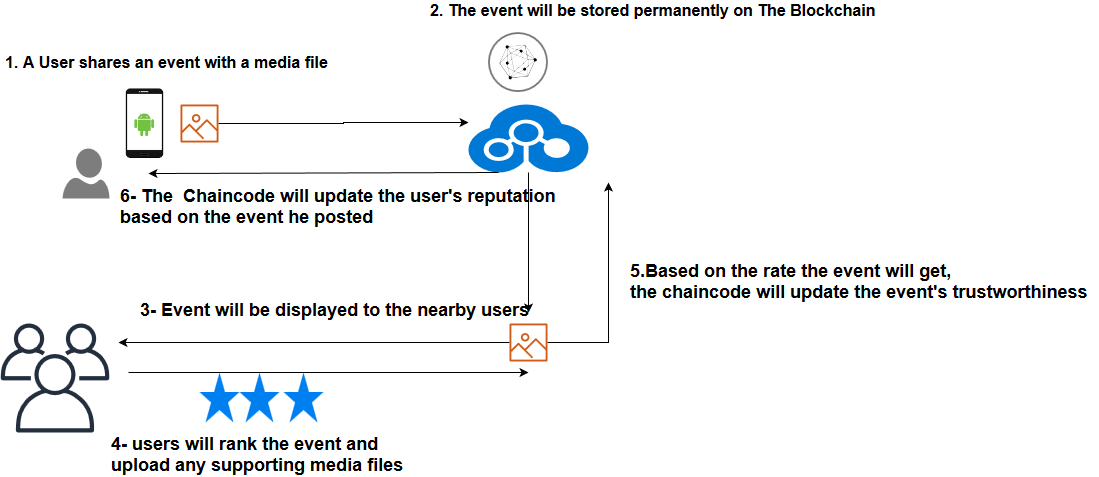
\includegraphics[width=15cm,height=5cm]{images/appflow.png}
	\caption{The Application Walkthrough}
	\label{fig:appflow}
	\end{figure}

\section{Architecture}
The platform would be dismantled into three main components: 
\begin{itemize}
  \item The Hyperledger fabric network.
  \item The Backend and Fabric SDK. 
  \item The Android Development. 
\end{itemize}

We will discuss every single component in details in a separate chapter we will start with the necessary background information about the Blockchain and main components and terms of hyper ledger fabric for example peers, chaincode, transaction ..etc. \\ Then we will discuss the backend, API Design  and how the API call requests will be consumed and the nodejs SDK handles the request, then forwards it to the chaincode which is the only way to interact with the blockchain.
Finally, we will discuss the Android application design, UI elements , network request in json that is calling API and the coding in depth with all the functions implemented \hyperref[fig:architecture]{Figure 2} depicts all the architecture overview of the platform. 
\begin{figure}[H]
	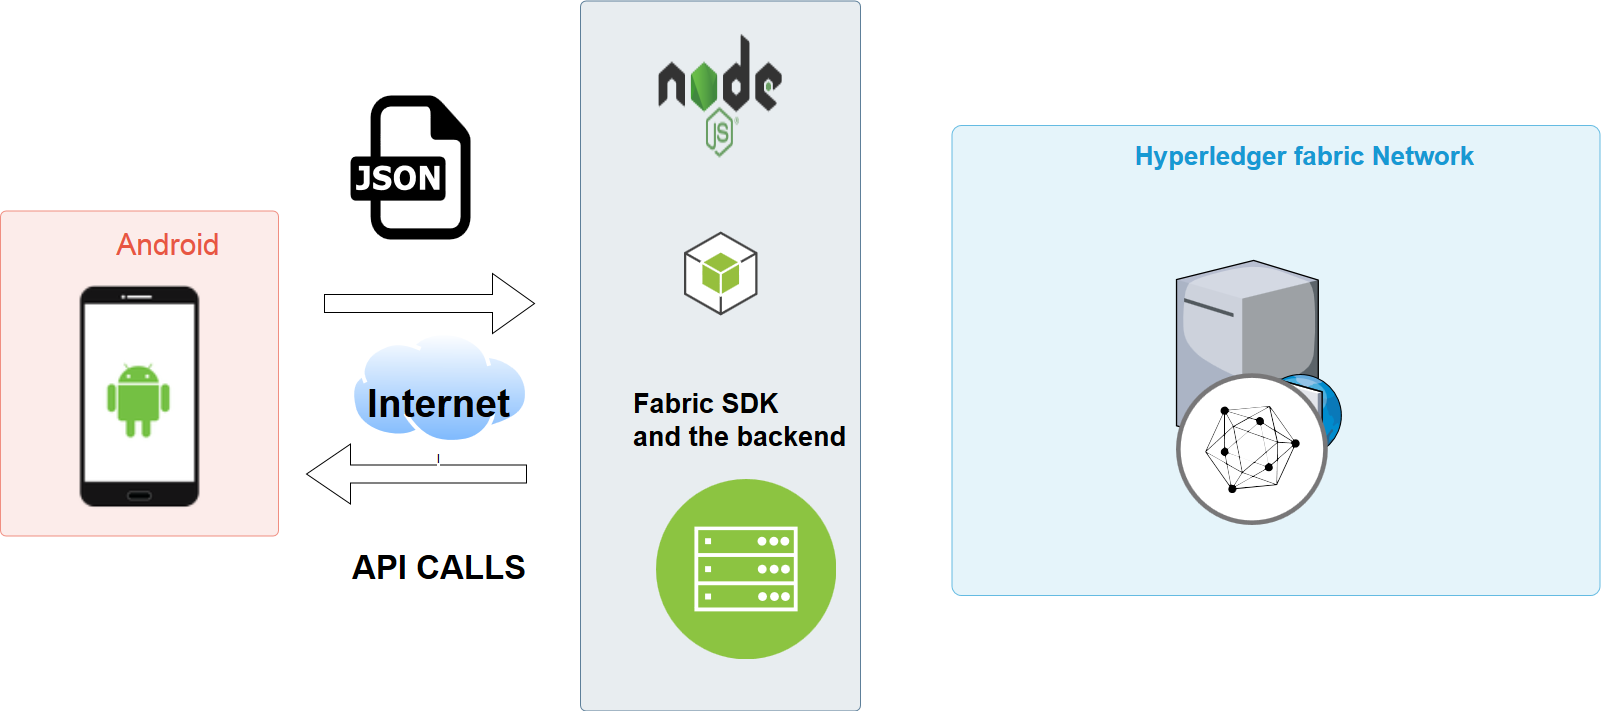
\includegraphics[width=15cm,height=10cm]{images/architecture.png}
	\caption{Architecture Overview}
	\label{fig:architecture}
	\end{figure}

      

 


      
\chapter{The Blockchain And Hyperledger Fabric Background}


\section{The Blockchain} 


 Blockchain has become one of the most hyped technology trend. it provides a new way of manging and storing data, in addition it provides capabilities for solving complex computing solutions. Taken further blockchain could be a cornerstone for secure data transfer and exchange on the internet.
Trust on the internet considered on the most stuborn problem, and here blockchain came to play. unlike the traditional database that requires a central authority which authorize the access to it and determine what is inserted and deleted. Traditional database has more two major flaws. 
First it has a single point of failure, in addition it will have only one major central autority. Central authority bewteen many stake holder levies additional overhead. 
For instance processing time and cost, vunerability and limitated participation between parties.  
Blockchain introduces a new way of storing data instead of a central sever the data will be stored on every single node on the network in a distributed fashion. 
\\

It's worth mentioning that Blockchain was based on a collection of related technologies, for instance, The public key infrastructure or PKI.
Public Key Infrastructure provides an infrastructure for digital certificate management. using the
aforementioned Cryptography techniques. using PKI will add Trustworthiness of the keys, thus we
can avoid a situation when Anybody could have uploaded their own keys and claimed they belong
to an email address (masquerading). After the organization generates the public and private key
it will share the public key and here comes the role of a digital signature, which is equivalent of
a handwritten signature, but offering far more inherent security, a digital signature is intended to
solve the problem of tampering and impersonation in digital communications. Digital signatures can
provide the added assurances of evidence to an origin, identity, and status of an electronic document,
transaction or message, as well as acknowledging informed consent by the signer. \\


in addition, it's also beneficial to cover some terms. 
A nonce is a number that is used once and never used again it helps to avoid duplicate transactions in digital transmission, for example, sometimes the data entered the database may have the same identifier adding nonce making it a bit harder for occasional replication. 
A Hash function is a mathematical process that taks data of any size and returns a unique hash with a fixed size no matter the size of the input data, however, it's only a one-way function thus it's hard to generate the original text from the hashed value. one major advantage of hashing is to keep the database small, as storing only the hash value save a tremendous amount of disk. in blockchain, hashes are used as an identifier for blocks and transactions. \\ 

Blockchain is a distributed database and its entries are immutable in other words it's not living on one server it's distributed and the data stored in it can't be modified or deleted. In traditional database data is stored in tables, rows and, columns usually in every table the stored data is related. 
For instance, a table might contain a customer's name and address. It will also contain a unique key for every record to link one table to another.
In a client-server model, the database usually lives on a single logical server and it's queried as request and the server runs the query and sends back the result to the client. Another aspect of this is in web architecture there are usually other tiers like a client, web server and load balancer, web servers and database servers are distributed among physical servers, however, logically they are governed by the same set of rules and said to be centralized even if they are physically distributed. the traditional database is useful however it's also vulnerable.
A blockchain database is structured in a way that it comprises of specific blocks of data organized in a specific structure, However, there is a huge difference in how the database is hosted a copy of a blockchain database resides on every node participate in the network there is no central server and it's not hierarchical it's a peer to peer. For example, if a user joins a blockchain environment all the database will be downloaded to his computer next each transaction happens on the blockchain will be recorded in every instance of the blockchain database in this way it's called a distributed Ledger. 
for every transaction, consensus must be reached by all participating nodes.
Lastly, a blockchain distributed ledger is immutable entries made will never be edited once a transaction occurred it will always be there. there is no remedy.  \\ 
 \hyperref[fig:bcvsdb]{Figure 2.1} depicts the main characteristics of the blockchain and the differences between the traditional databases.
\begin{figure}[H]
	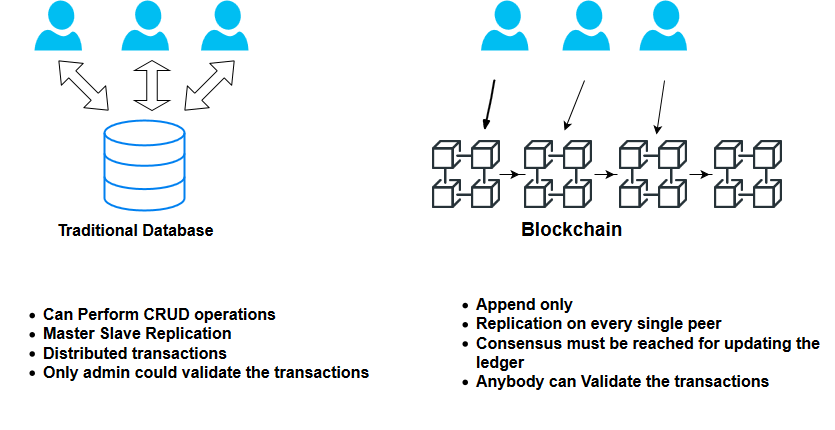
\includegraphics[width=15cm,height=10cm]{images/bcvsdb.png}
	\caption{Blockchain VS Traditional Database}
	\label{fig:bcvsdb}
	\end{figure}



\section{Hyperledger Fabric}
 
\subsection{Introduction}
Hyperledger Fabric is an Open-source permissioned Blockchain platform it was profounded under the Linux Foundation. Hyperledger Fabric became on of the most fastest growing project in the Linux Foundation. 
Hyperledger Fabric is the first platform that supports developing the smart contracts("chaincode") in general-purpose programming languages such as Java, Go and Node.js.
Furthermore, it's a permissioned blockchain in a simplified way this means the participants will be known to each other instead of being anonymous and fully untrusted. unlike permissionless which mainly relies on the miner to validate the transaction to relief the absence of trust. 
It provides a way to secure the interactions between different parties, which they not particularly trusting  each other having that it reinforces the trust between different entities.
Hypeledger Fabric is an enterprise distributed ledger based on GO programming language that uses smart contracts. 

Hyperledger Fabric came with a new concept that eliminates the mining concept, However it maintains all the characteristics of the blockchain, for instance, block immutability, order of operation determinism and the main benefits is the throughput of the system with huge number of transactions per minute by eliminating the concept of mining, also the consensus algorithm has the same properties as cryptocurrency blockchain. \\ 

Hyperledger is distributed by design there is no single point of failure or a single place that the information is stored.
all the participants are holding the same data, moreover, the data cannot be altered, thus hyperledger fabric reinforces the trust. 
Inside the blockchain, there is a ledger which stores every single operation occurred on the network. 
for example, imagine that there is a use case that we need to protect the copyright of some digital photos. and mistakenly we assigned a record of a photo to a wrong user and added the record to the ledger as a transaction. we couldn't delete this transaction, it will be always there and we have to assign the photo to the correct user. in essence, all the history of operations will be kept on the ledger, thus we could verify the all-time history of photos ownership by validating all the related transactions with the order of operation by replaying all the record inside the ledger you could find the latest world state,the world state or the final state of the data in our example the photo latest ownership will be the same amongst all network nodes, and due to the fact that the source of data is cryptographically signed that guarantees that the result of the data is the same trusted and unaltered. \\ 

Hyperledger Fabric could be integrated at any part of the network could serve the purpose publically or privately no matter it's physically located it will serve the purpose thanks to its flexibility t will fit and easily integrate within any system. \\ 


\subsection{Hyperledger Fabric Components} 

Hyperledger Fabric comprises of three main components:
\begin{itemize}
  \item Fabric Certificate Authority Fabric CA 
  \item Fabric Peer 
  \item Fabric Orderer 
\end{itemize} 


\textbf{ Fabric Certificate Authority (Fabric CA):} every single operation on hyperledger fabric must be signed with certificates no matter where the certificate came from if it is generated or purchased or generated from a trusted third party. Certificates are following X509 Standard and as mentioned there are many ways to generate certificates.
Fabric CA is a high-quality tool that pursues cryptographic standards to generate certificates these certificates are per user and attributes could be added while generating those certificates thus specific rules and permissions could be enforced per specific group of users. it is a place to generate certificates and  where the account would be created this process called enrollment you provide username and password and the fabric CA does all the magic. 
In addition fabric CA could be attached to an existing LDAP and all attributes would be fetched from there. 
by registering user and enroll them then provididing the certificate to SDK and the SDK signs all requests that will be executed inside hyperledger fabric. \\ 

\textbf{Peer:} is the place where the ledger blockchain is stored there could be more than one peer especially in production they contain the same ledger.  the request is sent from the SDK to peers, in order to do operations on the ledger like insert or query.  The main role of the peer is to endorse and update the ledger. all peers are synced automatically adding more peers in the network the other peer will automatically update the state of the newly joined peer, and this is facilitating the scalability of hyperledger fabric.  \\ 

\textbf{Orderer:} is coming into the heart of the consensus algorithm its main role is to provide order of operation before anything committed to the ledger it should be first validated and verified by the order and orderer creates the blocks so all transactions are stored into blocks and once blocks are full it will be sent to peers to be committed into the ledger. namely, the orderer is responsible for determining the order of operations.
There are several different implementations of ordering the first type is Solo which is mainly for development and this is only one instance if this instance fails all the operations for updating the ledger will fail, and the second type is Kafka which is used for production it's a distributed ordering service operation. \\

It's also worth mentioning \textbf{the channel} concept channels are a method developed in hyperledger fabric for data isolation More broadly it's a completely isolated instance of hyperledger fabric. every channel is completely independent and they never exchange data. when building network peers must be a part of the channel when creating peers, the peers should join a channel. with channel concept, the privacy and confidentiality of the data will be assured. the channel should be created and configured by a specific tool from hyper ledger fabric. in addition, one peer could be a part of different channels.  \\
 

\textbf{Chaincode} is a smart contract which is a program that reads and updates the ledger data, usually, all the business logic is written inside the chaincode. namely, the only way of interacting with the ledger will be only via the chaincode. 
The chaincode could be written in general purpose programming languages like Go, Java, and Javascript. There is no limitation on what could be done using chaincode it could have any desired complex business logic. \\

One important note that the chaincode must be apart of a channel inside one channel there could be as many as chaincodes. it could be possible to define all the business logic on one chaincode or split it amongst many chaincodes. 
The chaincode has to be installed and later instantiated. when writing chaincode it must be installed on every single peer that is a part of that channel this could be done using SDK or by using the peer itself. \\
 
Installing the chaincode on the peers is a must once it's the only way to interact with the ledger which resides on the peers. 
Once the chaincode is installed it should be then instantiated. 
Instantiating the chaincode will start a container that runs the chaincode while instantiating the chaincode the endorsement policy would be applied which will be responsible for validating and matching the rule on every single operation. For instance, applying a rule in a way  that for every transaction every peer must agree on adding the record otherwise the transaction will be rejected. \\  \\  \\ 
 
\textbf{Memebership Service Provider MSP}: is one of the most fundamental concepts of hyperledger fabric is a setup of cryptographical materials where the organizations will be defined. every single on hyperledger fabric must have its cryptographic certificates that define if a specific node belongs to specific organization generating the cryptographic material is trivial by hyperledger fabric tool cryptogen. 
The most essential part is that only peers that are part of the same MSP could communicate with each other. other peers couldn't the peer must be a part of the organization and this is defined by the peer's certificate later when configuring the channel all the public certificates will be shared on the configuration thus only the configured peer with a shared certificate could communicate and be a part of this channel. 

\textbf{The State Database:} In the blockchain concept, the state of the data would be tracked from the transactions history, for instance, assume that there is a simple balance transfer network. Person A sends 100 euros to person B and person C sends another 100 euros to person C. the current balance of person B should be 200 euros however the blockchain is just a serious of transaction in order to calculate the latest state of the accounts all transactions history should be reviewed and validated. thus for more efficient way hyper ledger fabric uses key-value store database to update the latest state of the data in an efficient way.
Chaincode invocations execute transactions against the current state data. To make these chaincode interactions extremely efficient, the latest values of all keys are stored in a state database. The state database is simply an indexed view into the chain?s transaction log, it can, therefore, be regenerated from the chain at any time. The state database will automatically get recovered (or generated if needed) upon peer startup before transactions are accepted.

State database options include LevelDB and CouchDB. LevelDB is the default state database embedded in the peer process and stores chaincode data as key-value pairs. CouchDB is an optional alternative external state database that provides addition query support when your chaincode data is modeled as JSON, permitting rich queries of the JSON content. See CouchDB as the State Database for more information on CouchDB.


\cleardoublepage

\subsection{Under The hood Hyperledger Fabric }

In this part, we will try to explain how hyperledger fabric works under the hood,
assume that we wanted to exchange the ownership of some assets, and The client wants to make a transaction, for example, adding data to the ledger. 
The first step is that the user has to register and enroll in the organization using fabric CA and get back the proper cryptographic materials that authorize him to interact with the network. Then the SDK will be responsible for preparing the transaction as a transaction proposal. This transaction will be sent to one or more peers. 
at this point the peer accepts this proposal and simulates it, the result of this simulation will be called read and write sets. at this phase, the ledger is not updated and the assets values remaining the same. 
The endorsing peers which are special kind of peers that its role is to verify and approve the transaction. this is will be done by validating the format and the signature of the transaction, and if the application user is authorized to make this transaction. 
then the peers are sending back those transaction responses to the SDK. the SDK collects all these transaction responses and signs it and send it to the orderer, the orderer node verifies the transaction signature and the endorsement policy. no matter if the transaction approved or rejected it will be stored on the blockchain, however, the state of the ledger will not be updated in case of the failure. in addition the order will verify the read and write sets collected from every single peer and makes sure they are all the same. 
Finally in case of the transaction is valid the orderer will send the transaction to the committing peers to be committed and updating the ledger.
\hyperref[fig:transactionflow]{Figure 2.2} depicts Hyperledger fabric transaction flow [1]. 
\begin{figure}[H]
	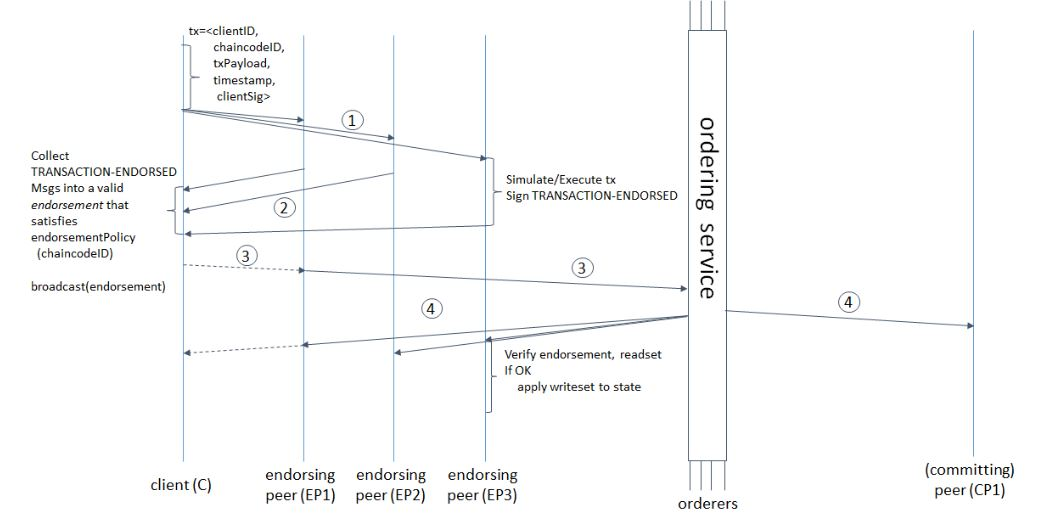
\includegraphics[width=15cm,height=10cm]{images/transactionflow.jpg}
	\caption{Hyperledger Fabric Transaction Flow Diagram}
	\label{fig:transactionflow}
	\end{figure}

 
 

 
 

 
 





 



 
  
\chapter{The Application Infrastructure}

The Fake news detetction system architecture is shown in\hyperref[fig:infrastructure]{Figure 3.1} it was inspired from balance transfer network [2]
 \begin{figure}[H]
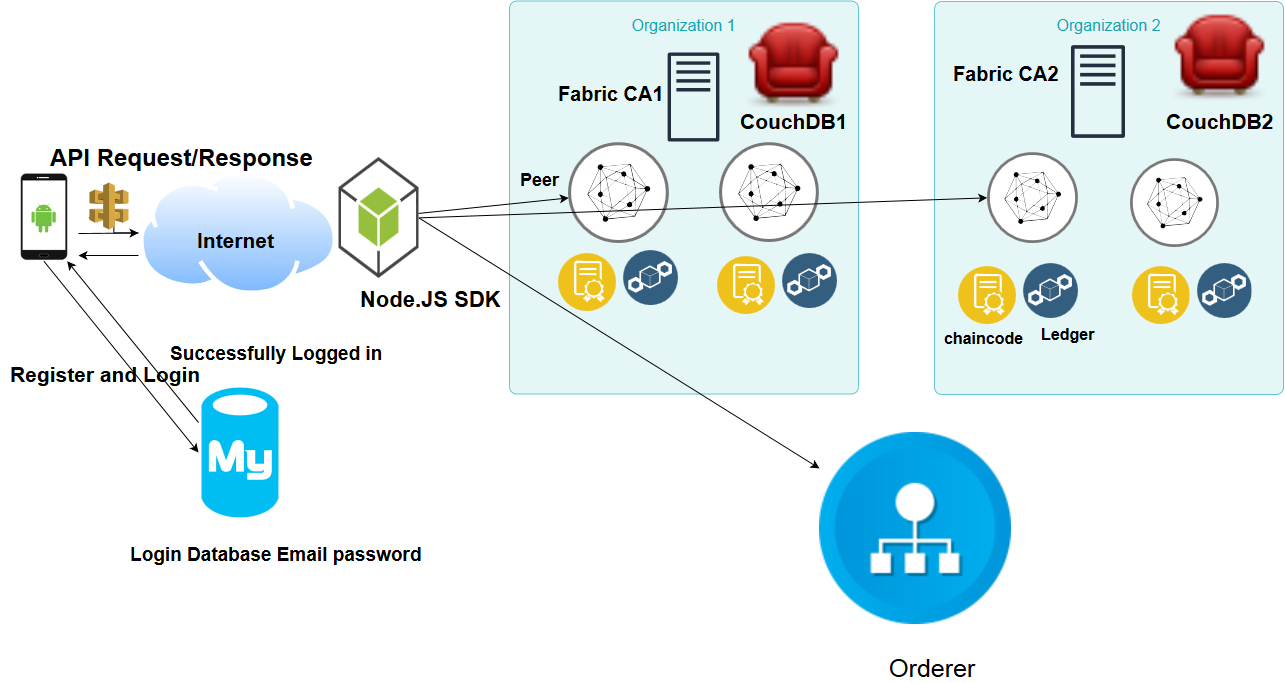
\includegraphics[width=15cm,height=12cm]{images/infrastructure.png}
\caption{The Application Infrastructure Overview}
\label{fig:infrastructure}
\end{figure}
\cleardoublepage

As shown the system comprises of Two Organizations Organization 1 and organization 2. with two peers in each organization. 
With a solo orderer node.  There are also two fabric CA Server one for each organization, a couchdb instance per organization for more efficient and rich queries. 
In addition, we are using node.js SDK  for interacting to the hyperledger fabric network and abstracting all the network infrastructure as a standard model thus the network could be scalable horizontally and vertically. All nodes are running on Docker containers for our testing purpose we implemented all the infrastructure on one Virtual Machine, However, in a production scenario every node should be an independent physical instance. \\ 

A layer of authentication using a traditional database was added, so that the users could sign up on our application using the traditional way we used email and password, however integrating a phone authentication with One time pad could be a trivial thing. 
Once the user successfully login he could send requests from android device using our application to the SDK. and the SDK will handle the interaction with hyperledger fabric network and the chaincode. 
 
The fabirc CA Server will be responsilbe for Registration of identities, Issuance of Enrollment Certificates for signing and identifying, Issuance of Transaction Certificates and Providing both anonymity and unlinkability when transacting on a Hyperledger Fabric blockchain. All these functionality are provided.
The network was an adoption of Balance transfer [2] A sample Node.js app to demonstrate fabric-client, fabric-ca-client and Node.js SDK APIs. 
the main idea of the network is to demontsrate a simple use case app using hyperledger fabric in order to transfer a balance from a user to another one and query the chaincode. we modified te network, added a couchdatabse instance and updating it with our chaincode. we modified the nodejs application to suit our application. 

Crypto material has been generated using the cryptogen tool from Hyperledger Fabric and mounted to all peers, the orderering node and CA containers. 
Beside An Orderer genesis block (genesis.block) and channel configuration transaction (mychannel.tx) has been pre generated using the configtxgen tool from Hyperledger Fabric and placed within the artifacts folder. 



\section{} 


 



 
  
\chapter{Android Application}
\section {Overview}
The application was designed to allow the users to interact with the blockchain. The Application UI was made similar to modern social networks, displaying the nearby events as a scrollable home feed \hyperref[fig:appscreens]{Figure 4.1} shows the different screens design of the Android app.  Authentication is required for the user to login to the blockchain network and to use the app. Once the user successfully authenticated the application will display the nearby events and the app is self-explanatory.

 \begin{figure}[H]
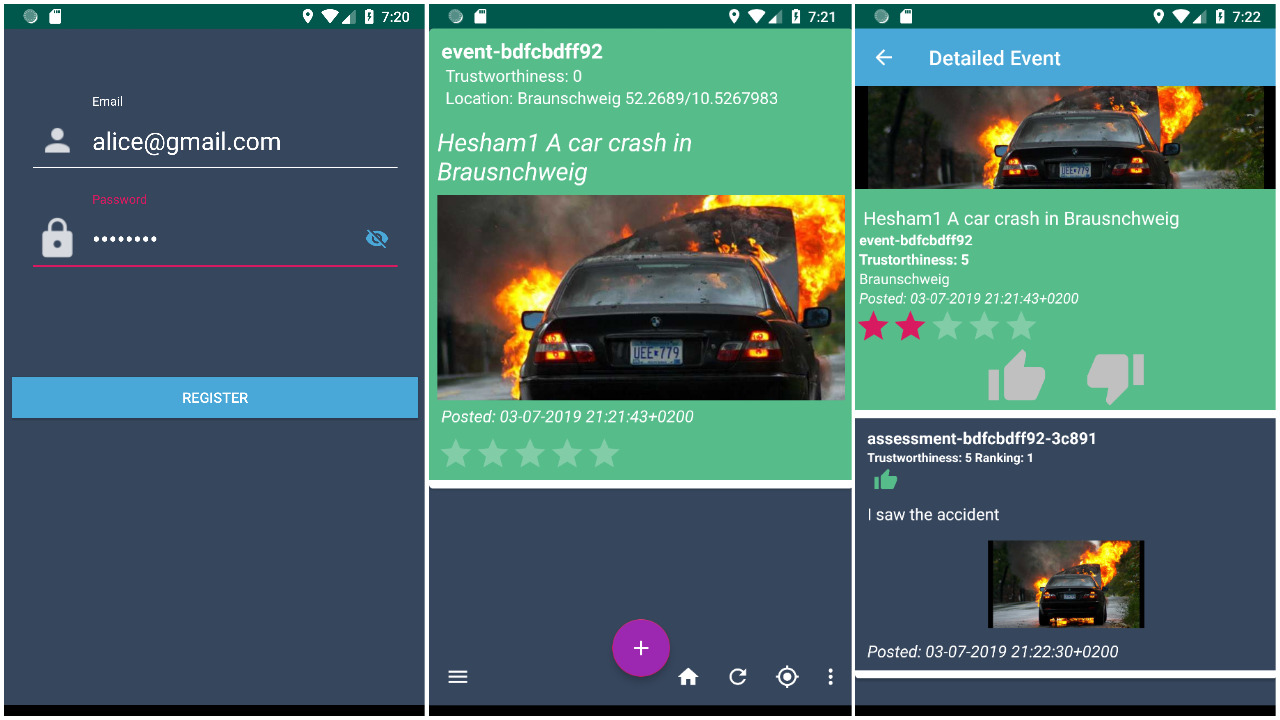
\includegraphics[width=15cm,height=10cm]{images/appscreens.jpg}
\caption{App Screens Represent The Application Design}
\label{fig:appscreens}
\end{figure}
 
\section{The Main Classes} 

In this section, we describe the main classes we used in the application. Every class provided a different functionality.
\subsection{Mainactivity}
MainActivity is the first activity launched when the application started. it checks if the user logged-in then it will direct the user to registration and login activities. 
Once the user login the email address will be stored in the shared-preference in order to keep the user login. The location access permission will be checked as it's one of the essential parts to continuously fetch the location of the users. A warning message will be displayed to the user if the location access wasn't granted. As long as the location access permission is granted. An enrollment request will be sent using the user's email address as discussed in 3.6 following the enrollment procedures and storing the JWT for making the upcoming requests to the blockchain network.
Finally, the application will use the JWT and the user's location to query the ledger and fetch all the nearby events and displaying them one by one chronologically in the news feed. 
Displaying the feed is nontrivial we used RecyclerView adapter which is an android class used to represent the data dynamically in a separate view and provides the ability to implement both horizontal and vertical layouts. The RecyclerView adapter used to display the data collections whose elements change at runtime based on user action or network events.  In other words every time we query the ledger the user get a JSON response containing all events list. Those events change at run time based on the user's location. The events will be displayed one by one in a separate view similar to Facebook or Instagram posts. 
We created a simple view holder for every event object and we instantiated an object of this view holder and binding the event data to it.    
The same methodology used to display the assessments list.
\hyperref[fig:mainactivityflow]{Figure 4.2} Describes the flow of the Mainactivity. 
 \begin{figure}[H]
\center
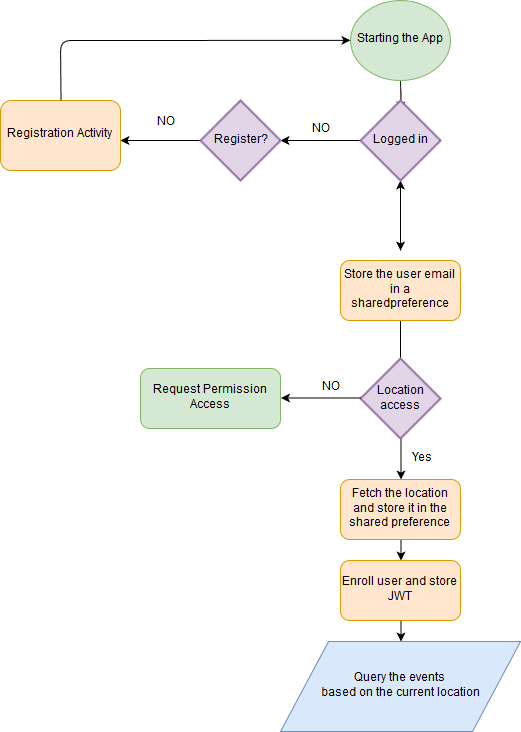
\includegraphics[width=10cm,height=9cm]{images/mainactivityflow.png}
\caption{Mainactivity Flowchart}
\label{fig:mainactivityflow}
\end{figure}

\subsection{AddEvent}
AddEvent is the activity that runs when the user wanted to create a new event. It will prompt the user to upload a photo and an event description. the activity will check the storage's permission access, and if it's granted it will allow the user to select an image from the gallery, then the image will be captured as a bitmap and converted into a string. This string will be hashed and sent to the Xampp server which will rebuild the media file and storing the file with its hash name. In other words, the picture will be stored with its hash and only the hash will be stored on the blockchain for fetching the picture and displaying it directly from the server, not from the blockchain. lastly, the transaction will be invoked by calling addEvent chaincode function name and passing all event's details as parameters.
If the transaction successfully invoked a confirmation message will be displayed to the user that the event is online, Otherwise, an error will be displayed. 
 Storing the hash instead of the entire media file will be more efficient as the file will be replicated many times on the peers.
It's similar to using A content delivery network CDN which is a standard way to deliver content more quickly and efficiently, based on their geographic location. A content delivery network CDN facilitates the quick transfer of assets needed for loading media content including images, and videos. using this approach will increase the performance and decrease the latency. In addition, storing the hash only will save a lot of disk space and assuring that the ledger size will be only a few megabytes instead of hundreds of terabytes. 
   
\hyperref[fig:mainactivityflow]{Figure 4.3} Describes the flow of AddingEvent Activity. 
 \begin{figure}[H]
\center
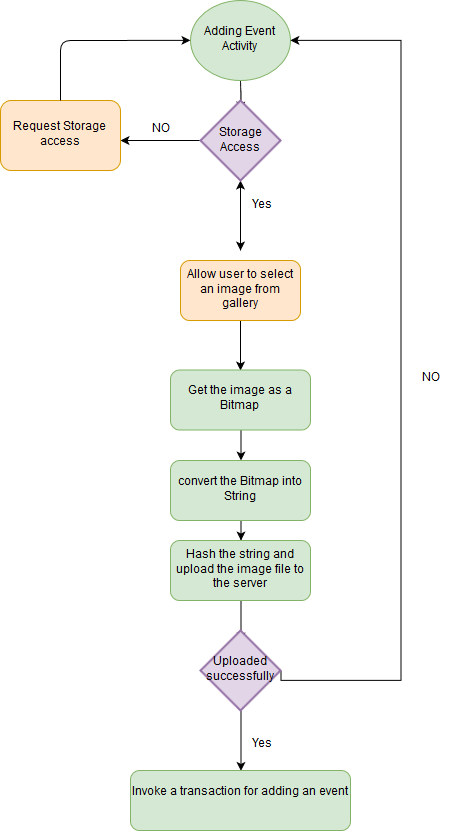
\includegraphics[width=8cm,height=12cm]{images/addingeventflowchart.png}
\caption{Addevent Flowchart}
\label{fig:addingeventflowchart}
\end{figure}

\cleardoublepage

\subsection{The Hashing Method}
For a more efficient way of storing data on the blockchain, only the media file is hashed and only the hash of it will be stored on CDN like S3 we store the data on a simple Xampp server for development purpose. the media file will be easily fetched and displayed. 
\textbf{PBKDF2} Algorithm is implemented. this hash function is slow enough to impede attacks, but still fast enough to not cause a noticeable delay for the users. A simple implementation of the hashing algorithm in listing 4.1.

 \begin{lstlisting}[caption={PBKDF2 Simple Implementation},captionpos=b]
import javax.crypto.SecretKeyFactory;
import javax.crypto.spec.PBEKeySpec;
import java.math.BigInteger;

public class Hashing {

    private static final int ITERATIONS = 1000;
    private static final int KEY_LENGTH = 192; // bits
    public static final String SALT = "Random Salt" ;

    public static String hashPassword(String password, String salt){
        char[] passwordChars = password.toCharArray();
        byte[] saltBytes = salt.getBytes();
        PBEKeySpec spec = new PBEKeySpec(
                passwordChars,
                saltBytes,
                ITERATIONS,
                KEY_LENGTH
        );
        SecretKeyFactory key = null;
        try {
            key = SecretKeyFactory.getInstance("PBKDF2WithHmacSHA1");
        } catch (NoSuchAlgorithmException e) {
            e.printStackTrace();
        }
        byte[] hashedPassword = new byte[0];
        try {
            hashedPassword = key.generateSecret(spec).getEncoded();
        } catch (InvalidKeySpecException e) {
            e.printStackTrace();
        }
        return String.format("%x", new BigInteger(hashedPassword));
    }
}
\end{lstlisting}
\cleardoublepage


\subsection{Voting}
When the user selects on a specific event a new activity will be created, and the event will be separately displayed with more details about the event, and the application will allow the user to judge or assess the event by up-voting or down-voting, also it would be possible to attach a description or a media file.
The voting activity is similar to adding an event the data will be stored captured media file will be hashed and uploaded to the server and finally, a transaction will be invoked and judgeEvent chaincode function will be invoked and all assessments details will be passed as parameters. in the end, a confirmation message will be displayed in case of success and an error in case of any failure or network error. 
Assessing events will credit or discredit a specific event and directly reflects the creator of the event's reputation score. 
The voting is similar to adding the event activity just different in calling the judgeEvent. 


\subsection{Login and Register}
In order to allow the users to log-in and register, we implemented two separate activities. the user will input an email and password, then we are validating the user input. and an error will be displayed if the email address is not valid or empty or in use by another user. 
If the data was valid we submit a request over the network and store it to the relational database. The email will be stored in a plain text, however, the password will be stored hashed. 
Similarly, the login activity once the user inputs his email and password it will be checked against the database if the credentials were correct the access is granted to the user and the email will be saved to keep the user logged in.

\cleardoublepage

\subsection{Ranking and Trustworithness} 

One of the main features we introduced is ranking the events and calculating users' reputation.
The user's reputation will depend on the user's interaction on the platform. how frequent he participated, how many good reviews he received on the event he created. 
Every user starts with 0 reputation score. Adding an event will increase his score by +1.  \\
The algorithm considers the users rank and location's trustworthiness or how close is the user from the event.
Assume a user with score 510 and was about 10 meters away from an event he is going to assess. First, we convert the score into stars as the user's reputation score is 510 then the stars function will return 5. Second, we calculate how far is the user and return a value from 1 (almost in the scene of the event he is assessing)  to .1 (so far away from the event) in this case the closeness function will emit 1 so the final score the user is 25. This score will increase/decrease in the assessed event's trustworthiness. Depending on the vote type if it's up/down vote this will credit or discredit the event's trustworthiness and increase or decrease the overall reputation score of the event creator. 
Once the assessment is made the chaincode updates the assessed event's trustworthiness and the event creator's reputation score.
In summary, What easily influences the user’s reputation and the event's trustworthiness is getting good/bad reviews from the highly ranked users who are very nearby to the assessed event. 
\hyperref[fig:mainactivityflow]{Figure 4.4} describes the ranking algorithm. 
 \begin{figure}[H]
\center
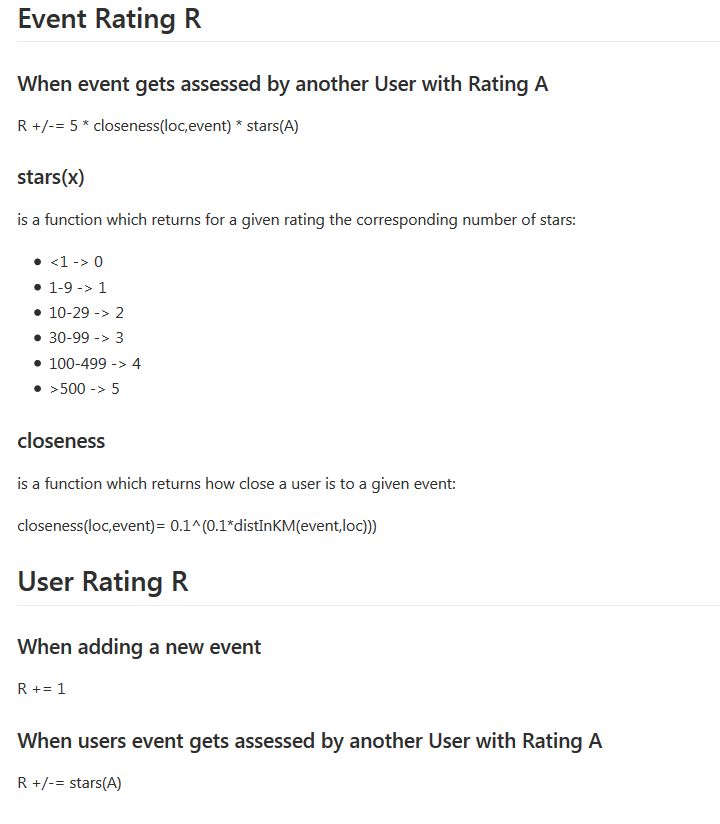
\includegraphics[width=14cm,height=13cm]{images/ranking.png}
\caption{The Ranking Algorithm}
\label{fig:ranking}
\end{figure}
 
\chapter{Issues and Future Work}


\section{Issues} 
One of the design issues faced during the development is where should the SDK be installed from Architecture point of view?
1-On the server side where the hyperledger fabric lives?  or 2-On the client side (Android side) taking into consideration there is no official support for an Android SDK. The only supported SDKs are on GO, javascript, and java.
Building and integrating an Android SDK from scratch is nontrivial it will require such time and effort and a dedicated team to achieve this goal.   
We implemented the SDK on the server side where Hyperledger fabric lives, thus we are obscuring the network and only exposing the node.js App with all scripts that consume the requests and make SDK calls to interact with the ledger. Designing the backend that way by totally obscuring the hyperledger fabric network will have the following advantages: 

\begin{enumerate}
  \item Since there is no officially supported SDK for Android it will require much time and effort to redevelop an Android SDK, as there is no point for reinventing the wheel. 
  \item Standardizing the communication using APIs. this way all the APIs could be easily standardized and manifested, Meaning, the application will only call a fixed URL, chaincode function name and passing arguments. No matter on which language the application was written if the client was written on android, web, or ios. It will be the same network rest API call made over the internet a example discussed in 3.7. However, if the SDK lives on the client side the application developer will be responsible for customizing the requests to match the SDK's language, and the way it interacts with the hyperledger fabric network.      
  \item Avoiding the latency and restricting all the transaction flow on the internal network. so the communication between the SDK and the peers will be done on the internal network and we avoid the delay will be introduced if the requests were made on the internet with many hobs
  \item The communication will be encrypted using SSL certificate. All the header and payload will be encrypted.
  \item The Whole hyperledger fabric network will be isolated and couldn't be directly accessed from the internet as we only exposing the end point for communication and no direct interaction with the peers, orderer or Fabric CA They are hidden behind the node.js App. in case of the node.js app compromised the data and all the hyeprledger fabric network will not be affected. 
  \item Finally, Avoiding the unnecessary SDK Library size which will expected to be around 30-50Mb on the smartphone taking into consideration the whole application size is 5Mb. 
\end{enumerate}
\clearpage
\noindent One main \textbf{disadvantage} of this approach is the data could be viewed by the server admin and this raises \textbf{privacy concerns}, as discussed on 3.7 the Android application is calling the exposed URL and passing the parameters required in order to make transactions.  Parameters passed such as the chaincode function name and the events details.
The node.js app scripts consumed those data and use the node.js SDK to do different operations on the fabric network such as querying the ledger or invoking a transaction. 
At the point, the data could be leaked by the server admin. even hyperledger fabric didn't explicitly discussed this concern and they implemented the Hyperledger Composer[8] that simply exposes the network on the same way using server and generating a REST API from a deployed blockchain business network that can be easily consumed by HTTP or REST clients.
This was the reason we wanted to install the SDK on the client side and making the requests directly to fabric network or run the node.js on an Intel SGX enclave. 
 However, to modify the data directly will be nontrivial. and could be easily investigated. Since the data on the ledger is append-only and the business logic is reinforced by the chaincode. Furthermore introducing a simple cryptographic scheme to cipher the data would resolve this issue. 
\hyperref[fig:enrollmentproc]{Figure 5.1} depicts how the network is obscured.  
\ \\
 \begin{figure}[H]
\center
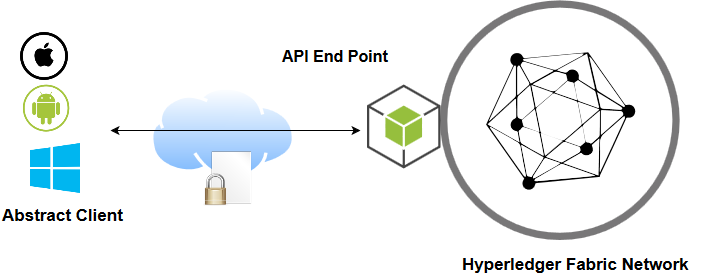
\includegraphics[width=10cm,height=8cm]{images/issues.png}
\caption{Obscuring the Network by Using the Node.js App }
\label{fig:issues}
\end{figure}

\section{Future Work} 

Based on our reusable and modular design we could adopt any complex business logic by simply modifying the chaincode. Furthermore, we could introduce more roles such as, Researchers and verifiers who could have more privileges like banning other users who scam the platform and prevent any malicious behavior. 
 

\chapter {Conclusion}

In this chapter, we conclude the work has been done in the research project and all tasks that have been accomplished.

\section{Summary}
During the research project, We aimed to implement a real solution leveraging the blockchain features such as decentralization and data immutability.
In addition, Providing a solution for a real problem like Fake news. As Fake news in the digital era is one of the latest issues that has raised many concerns and has many negative effects for instance, biasing the public opinion, spreading the hate speech and destroying innocent people's reputation. \\ 

\noindent We started by studying the blockchain and hyperledger fabric. We designed a case study scenario for a mobile application that incents users to share and rank stories and storing them on the blockchain. Hyperledger fabric was used as a permissioned blockchain that restricting the access into the network and only the verified entities could participate. \\ 
 
\noindent We built a fully functioned development network using Docker containers and adopt one of the provided node.js APP, which abstracts the whole network and exposes Rest APIs for different chaincode operations on the hyperledger fabric,The node.js App also serves as a back-end to the whole infrastructure after highly modifying the code to match our case. 
We built a simple Xampp development server in order to allow the users to register in a traditional way using email and password, Furthermore we introduced an efficient way for storing data on the blockchain by storing only the hash of the media files, and serving the media files as content delivery network CDN approach for more efficient, low latency and high performance. 
In addition, We implemented a score and reputation system using the chaincode and location trustworthiness.  We designed an Android application for the end user that facilitates the interaction and allows different operations. The application designed to be user-friendly, self-explanatory and easy to use. Finally, we introduced a modular design thus more features with the minimum required modifications will be easy introduced and integrated into an inter-operable environment.

\addcontentsline{toc}{chapter}{Conclusion}

\cleardoublepage

\begin{thebibliography}{9}

\bibitem{latexcompanion}
Hyperledger Fabric architecture
\url{Hyperledger-fabric.readthedocs.io. “Architecture Explained”, Hyperledger-fabricdocs master documentation, 2017}
\bibitem{latexcompanion}
Hyperledger Fabric Balance transfer network 
\url{https://github.com/hyperledger/fabric-samples/tree/release-1.4/balance-transfer}
\bibitem{latexcompanion}
Hyperledger Fabric Node.js SDK
\url{https://fabric-sdk-node.github.io/release-1.4/index.html}
\bibitem{latexcompanion}
Node.js APP Source Code
\url{https://gitlab.ibr.cs.tu-bs.de/ds-thesis/2018-pa-hesham-mohamed-media-blockchain/tree/network-configurations/app}
\bibitem{latexcompanion}
Chaincode Rest API calls 
\url{https://gitlab.ibr.cs.tu-bs.de/ds-thesis/2018-pa-hesham-mohamed-media-blockchain/wikis/API-Calls-Documentation}
\bibitem{latexcompanion}
A guide for setting up the infrastructure
\url{https://gitlab.ibr.cs.tu-bs.de/ds-thesis/2018-pa-hesham-mohamed-media-blockchain/wikis/How-to-setup-the-infrastructure.}

\bibitem{latexcompanion}
Android Documentation
\url{https://developer.android.com/docs}
\bibitem{latexcompanion}
Hyperledger Composer REST Server
\url{https://hyperledger.github.io/composer/v0.19/reference/rest-server}

\bibitem{latexcompanion}
Bitcoin White Paper
\url{https://bitcoin.org/bitcoin.pdf}

\bibitem{latexcompanion}
Blockchain vs Tranditional Database
\url{https://www.researchgate.net/publication/327483781_Blockchain_Versus_Database_A_Critical_Analysis}

\bibitem{latexcompanion}
Blockchain Overview
\url{https://www.researchgate.net/publication/318131748_An_Overview_of_Blockchain_Technology_Architecture_Consensus_and_Future_Trends}

\bibitem{latexcompanion}
Hawk: The Blockchain Model of Cryptography and Privacy-Preserving Smart Contracts
\url{https://www.computer.org/csdl/proceedings-article/sp/2016/0824a839/12OmNs59JYD}

\bibitem{latexcompanion}
Hyperledger Fabric: A Distributed Operating System forPermissioned Blockchains
\url{https://arxiv.org/pdf/1801.10228.pdf}

\bibitem{latexcompanion}
All roads lead to Rome:Many ways to double spend your cryptocurrency
\url{https://arxiv.org/pdf/1811.06751.pdf}
\bibitem{latexcompanion}
Using CouchDB on Hyperledger Faric
\url{https://hyperledger-fabric.readthedocs.io/en/release-1.4/couchdb_tutorial.html}


\appendix
\end{thebibliography}
\cleardoublepage


\end{document}
 